\documentclass[a4paper,12pt]{report}
\usepackage[utf8]{inputenc}
\usepackage[czech]{babel}
\usepackage{amsmath}
\usepackage{geometry}
\usepackage{xcolor}
\usepackage{fancyhdr}
\usepackage{soul}
\usepackage{array}
\usepackage{pgf}
\usepackage[normalem]{ulem}
\usepackage{hyperref}
\usepackage[figurename=Obr.,tablename=Tab.]{caption}
\usepackage{graphicx}
\usepackage{pgffor}
\usepackage{placeins}
\usepackage[inline]{enumitem}
\usepackage{multirow}



\geometry{top=2.5cm, bottom=2.5cm, left=2.0cm, right=2.0cm}

% Variables, fill it here!
\newcommand{\studentName}{Bc. Pavel Mikula}
\newcommand{\studentID}  {MIK0486}
\newcommand{\teacherName}{Mgr. Pavla Dráždilová, Ph.D.}

\renewcommand{\headrulewidth}{0pt}
\renewcommand{\footrulewidth}{0pt}

% Table and Image references
\newcommand{\tabref}[1]{Tab. \ref{#1}}
\newcommand{\figref}[1]{Obr. \ref{#1}}

% Array commands
\newcommand{\av}[2]{%
    \pgfmathparse{{#1}[#2]}%
    \mbox{\pgfmathresult}%
}

\newcommand{\orderArrayNumbered}[1]{%
    (\av{#1}{0}, \av{#1}{5}, \av{#1}{6}, \av{#1}{7}, \av{#1}{8}, \av{#1}{9}, \av{#1}{10}, \av{#1}{11}, \av{#1}{12}, \av{#1}{1}, \av{#1}{2}, \av{#1}{3}, \av{#1}{4})%
}

% Type of table columns that orients text to center
\newcolumntype{P}[1]{>{\centering\arraybackslash}p{#1}}

\begin{document}
\thispagestyle{empty}
\setcounter{page}{0}

% Title and header section
\begin{center}
    
\includegraphics[width=0.8\textwidth]{assets/logo.png} \\[4em]
    \vspace{4em}
    \textbf{\huge{Petriho Sítě I}} \\
    \vspace{4em}
    \textbf{\large{Semestrální projekt - Řízení světelné křižovatky}} \\
\end{center}

% Student information, values are implemented in variable section above
\vspace{3em}
\hspace{2em}
\begin{tabular}{ll}
    \textbf{Jméno studentky/studenta:}  & \hspace{6em} \studentName \\[0.5em]
    \textbf{Osobní číslo:}              & \hspace{6em} \studentID   \\[0.5em]
    \textbf{Jméno cvičící/cvičícího:}   & \hspace{6em} \teacherName \\
\end{tabular}

% Footer section
\vspace{25em}
\begin{center}
    \textbf{Ostrava, AR 2024/2025}
\end{center}

\newpage
\section*{Úvod}
\label{sec:introduction}

Projekt představuje model semaforového řešení křižovatky využívající Petriho sítě.
Struktura PN systému zobrazuje dynamické řízení provozu na světelné křižovatce, kde se mohou pohybovat maximálně 3 vozidla současně.

Jednotlivá místa v modelu reprezentují možné stavy semaforů a fronty čekajících vozidel ve směrech sever-jih (SN) a východ-západ (WE).
Přechody mezi stavy symbolizují změnu barev jednotlivých semaforů a pohyb vozidel na křižovatce.
Model také zahrnuje bezpečnostní synchronizační prvky mezi jednotlivými směry, které zabraňují kolizím vozidel.

Počáteční značení se nachází ve stavu, kdy na jednom semaforu je zelená, na druhém červená a v křižovatce se nenachází žádné vozidla.
$M_0 = (3, 0, 1, 0, 0, 0, 0, 0, 0, 0, 1, 0, 1)$

\endinput
\section*{Návrh sítě}
\label{sec:network_design}

Pro popis jednotlivých stavů a přechodu na \figref{fig:network} bude využita zkratka $p_i$ pro místa a $t_i$ pro přechody, kde $i$ je identifikátor před dvojtečkou.

\begin{figure}[h!]
    \centering
    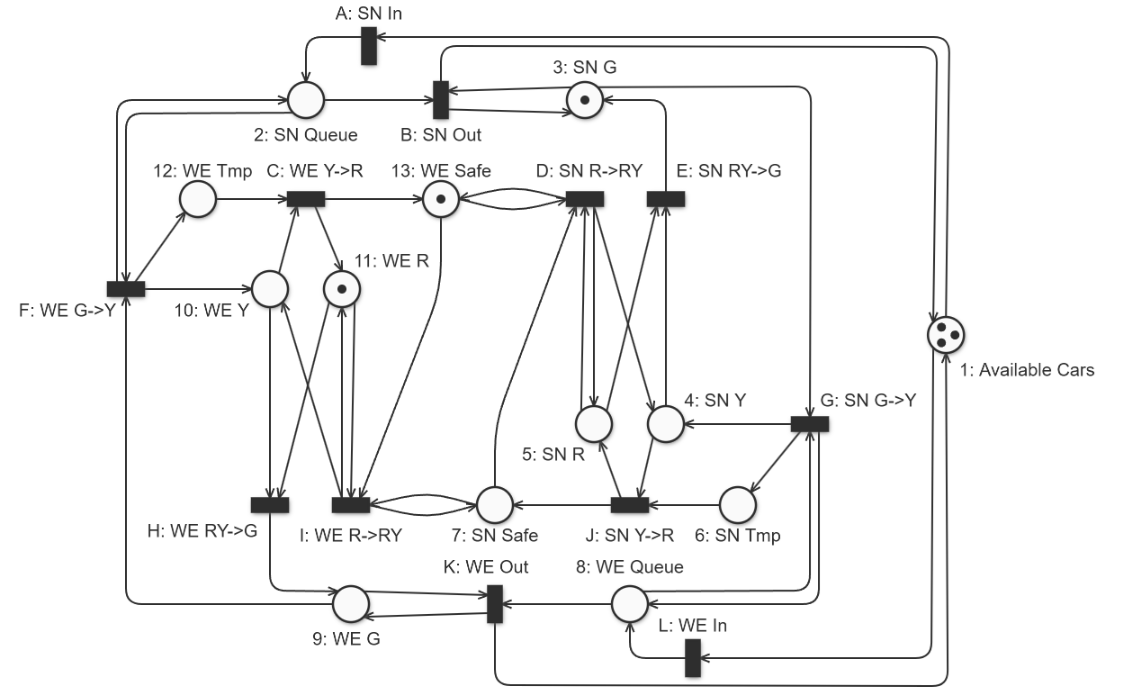
\includegraphics[width=0.85\textwidth]{assets/pes_network}
    \caption{Petriho síť reprezentující chování semaforů na křižovatce.}
    \label{fig:network}
\end{figure}

\begin{table}[h!]
    \centering
    \resizebox{0.50\textwidth}{!}{
        \begin{tabular}{c|c|c|c|c|c|c|c|c|c|c|c|c|}
            & \textbf{$t_a$} & \textbf{$t_b$} & \textbf{$t_c$} & \textbf{$t_d$} & \textbf{$t_e$} & \textbf{$t_f$} & \textbf{$t_g$} & \textbf{$t_h$} & \textbf{$t_i$} & \textbf{$t_j$} & \textbf{$t_k$} & \textbf{$t_l$} \\
            \hline
            %                  A      B      C      D      E      F      G      H      I      J      K      L
            \textbf{$p_1$}   & $-1$ & $+1$ & $  $ & $  $ & $  $ & $  $ & $  $ & $  $ & $  $ & $  $ & $+1$ & $-1$ \\
            \textbf{$p_2$}   & $+1$ & $-1$ & $  $ & $  $ & $  $ & $ 0$ & $  $ & $  $ & $  $ & $  $ & $  $ & $  $ \\
            \textbf{$p_3$}   & $  $ & $ 0$ & $  $ & $  $ & $+1$ & $  $ & $-1$ & $  $ & $  $ & $  $ & $  $ & $  $ \\
            \textbf{$p_4$}   & $  $ & $  $ & $  $ & $+1$ & $-1$ & $  $ & $+1$ & $  $ & $  $ & $-1$ & $  $ & $  $ \\
            \textbf{$p_5$}   & $  $ & $  $ & $  $ & $ 0$ & $-1$ & $  $ & $  $ & $  $ & $  $ & $+1$ & $  $ & $  $ \\
            \textbf{$p_6$}   & $  $ & $  $ & $  $ & $  $ & $  $ & $  $ & $+1$ & $  $ & $  $ & $-1$ & $  $ & $  $ \\
            \textbf{$p_7$}   & $  $ & $  $ & $  $ & $-1$ & $  $ & $  $ & $  $ & $  $ & $ 0$ & $+1$ & $  $ & $  $ \\
            \textbf{$p_8$}   & $  $ & $  $ & $  $ & $  $ & $  $ & $  $ & $ 0$ & $  $ & $  $ & $  $ & $-1$ & $+1$ \\
            \textbf{$p_9$}   & $  $ & $  $ & $  $ & $  $ & $  $ & $-1$ & $  $ & $+1$ & $  $ & $  $ & $ 0$ & $  $ \\
            \textbf{$p_{10}$} & $  $ & $  $ & $-1$ & $  $ & $  $ & $+1$ & $  $ & $-1$ & $+1$ & $  $ & $  $ & $  $ \\
            \textbf{$p_{11}$} & $  $ & $  $ & $+1$ & $  $ & $  $ & $  $ & $  $ & $-1$ & $ 0$ & $  $ & $  $ & $  $ \\
            \textbf{$p_{12}$} & $  $ & $  $ & $-1$ & $  $ & $  $ & $+1$ & $  $ & $  $ & $  $ & $  $ & $  $ & $  $ \\
            \textbf{$p_{13}$} & $  $ & $  $ & $+1$ & $ 0$ & $  $ & $  $ & $  $ & $  $ & $-1$ & $  $ & $  $ & $  $ \\
        \end{tabular}
    }
    \caption{Matice incidence Petriho sítě. \protect\footnotemark[1]{Aaaa}}
    \label{tab:transitions}
\end{table}

\footnotetext[1]{Hodnoty 0 představují obousměrnou výměnu tokenu mezi místem. Hodnoty +1 a -1 značí přidání nebo odebrání tokenu z místa.}

\endinput

\newpage
\section*{Popis sítě}
\label{sec:network_description}

Jednotlivá místa v modelu reprezentují možné stavy semaforů a fronty čekajících vozidel ve směrech sever-jih (SN) a východ-západ (WE).
Přechody mezi stavy symbolizují změnu barev jednotlivých semaforů a pohyb vozidel na křižovatce.
Model také zahrnuje bezpečnostní synchronizační prvky mezi jednotlivými směry, které zabraňují kolizím vozidel.

\subsection*{Místa}
\label{subsec:places}

Stavy zobrazeny v \tabref{tab:places-description} popisují možné stavy semaforů na křižovatce pro jednotlivé směry SN a WE. \\\\
$p_1$ - Limit pro maximální počet aut v křižovatce

\begin{table}[h!]
    \renewcommand{\arraystretch}{1.3}
    \resizebox{\textwidth}{!}{%
        \begin{tabular}{P{1cm}|P{1cm}|p{15cm}}
            \multicolumn{2}{P{2.5cm}|}{\textbf{Stav}} & \textbf{Popis} \\
            \hline
            SN & WE & \\
            \hline
            $p_2$ & $p_8$    & Fronta čekajících aut na zelenou                \\
            $p_3$ & $p_9$    & Zelená na semaforu                              \\
            $p_4$ & $p_{10}$ & Žlutá na semaforu                               \\
            $p_5$ & $p_{11}$ & Červená na semaforu                             \\
            $p_6$ & $p_{12}$ & Dočasný stav blokující přechod žluté do červené \\
            $p_7$ & $p_{13}$ & Zabezpečení střídání směrů                      \\
        \end{tabular}%
    }
    \caption{Tabulku popisu stavů semaforů na křižovatce.}
    \label{tab:places-description}
\end{table}

\subsection*{Přechody}
\label{subsec:transitions}

Obdobně jako u míst, přechody zobrazeny v \tabref{tab:transitions-description} popisují změny stavů semaforů na křižovatce pro jednotlivé směry SN a WE.

\begin{table}[h!]
    \renewcommand{\arraystretch}{1.3}
    \resizebox{\textwidth}{!}{%
        \begin{tabular}{P{1cm}|P{1cm}|p{15cm}}
            \multicolumn{2}{P{2.5cm}|}{\textbf{Přechod}} & \textbf{Popis} \\
            \hline
            SN & WE & \\
            \hline
            $t_A$ & $t_L$ & Příjezd auta ze směru S nebo W                   \\
            $t_B$ & $t_K$ & Odjezd auta ve směr N nebo E                     \\
            $t_F$ & $t_G$ & Změna stavu semaforu ze zelené na žlutou         \\
            $t_I$ & $t_J$ & Změna stavu semaforu ze žluté na červenou        \\
            $t_C$ & $t_I$ & Změna stavu semaforu z červené na žluto-červeno  \\
            $t_H$ & $t_E$ & Změna stavu semaforu ze žluto-červené na zelenou \\
        \end{tabular}%
    }
    \caption{Tabulku popisu přechodů semaforů na křižovatce.}
    \label{tab:transitions-description}
\end{table}

\endinput

\newpage
\section*{Graf dosažitelnosti}
\label{sec:reachability_graph}

\newcommand{\mO}   {1, 0, 1, 0, 1, 0, 1, 0, 0, 0, 0, 0, 0}
\newcommand{\mI}   {0, 0, 1, 0, 1, 0, 1, 0, 0, 0, 0, 1, 0}
\newcommand{\mII}  {0, 0, 1, 0, 1, 1, 1, 0, 0, 0, 0, 0, 0}
\newcommand{\mIII} {0, 0, 1, 0, 1, 0, 0, 1, 0, 1, 0, 1, 0}
\newcommand{\mIV}  {0, 0, 1, 0, 1, 0, 0, 0, 1, 0, 1, 1, 0}
\newcommand{\mV}   {0, 1, 1, 0, 0, 0, 0, 0, 1, 0, 1, 1, 0}
\newcommand{\mVI}  {0, 0, 1, 0, 1, 0, 0, 1, 1, 0, 0, 1, 0}
\newcommand{\mVII} {0, 0, 0, 0, 0, 0, 0, 0, 1, 0, 1, 1, 1}
\newcommand{\mVIII}{1, 0, 0, 0, 0, 0, 0, 0, 1, 0, 1, 0, 1}
\newcommand{\mIX}  {0, 0, 0, 0, 0, 1, 0, 0, 1, 0, 1, 0, 1}
\newcommand{\mX}   {0, 1, 0, 1, 0, 1, 0, 0, 1, 0, 1, 0, 0}
\newcommand{\mXI}  {0, 0, 1, 0, 1, 1, 0, 0, 1, 0, 1, 0, 0}
\newcommand{\mXII} {0, 1, 1, 0, 0, 1, 0, 0, 1, 0, 1, 0, 0}
\newcommand{\mXIII}{0, 0, 1, 0, 1, 1, 0, 1, 1, 0, 0, 0, 0}

Pro graf dosažitelnosti jsem zvolil verzi sítě (viz \figref{fig:network}) k-omezenou pro pouze 1 auto na křižovatce tedy $M_0$ = \orderArray{\mO}.

\begin{figure}[h!]
    \centering
    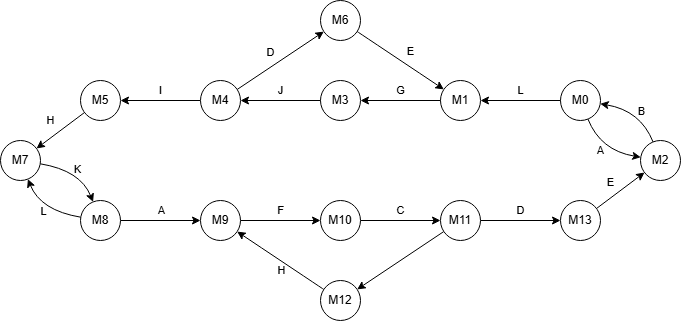
\includegraphics[width=0.85\textwidth]{assets/graphK1}
    \caption{Graf dosažitelnosti pro k-omezenou síť s jedním autem na křižovatce.}
    \label{fig:reachability_graph_k1}
\end{figure}

\newcommand{\convertArrayToColumn}[1]{%
    \av{\mO}{#1} & \av{\mI}{#1} & \av{\mII}{#1} & \av{\mIII}{#1} & \av{\mIV}{#1} & \av{\mV}{#1} & \av{\mVI}{#1} & \av{\mVII}{#1} & \av{\mVIII}{#1} & \av{\mIX}{#1} & \av{\mX}{#1} & \av{\mXI}{#1} & \av{\mXII}{#1} & \av{\mXIII}{#1}
}

\newcommand{\conn}[2]{%
    \overset{#1}{\xrightarrow{\hspace{0.2cm}}}M#2
}

\begin{table}[h!]
    \centering
    \resizebox{1.0\textwidth}{!}{
        \begin{tabular}{c|c|c|c|c|c|c|c|c|c|c|c|c|c|c}
                              & M0 & M1 & M2 & M3 & M4 & M5 & M6 & M7 & M8 & M9 & M10 & M11 & M12 & M13 \\
            \hline
            \textbf{$p_1$}    & \convertArrayToColumn{0} \\
            \textbf{$p_2$}    & \convertArrayToColumn{5} \\
            \textbf{$p_3$}    & \convertArrayToColumn{6} \\
            \textbf{$p_4$}    & \convertArrayToColumn{7} \\
            \textbf{$p_5$}    & \convertArrayToColumn{8} \\
            \textbf{$p_6$}    & \convertArrayToColumn{9} \\
            \textbf{$p_7$}    & \convertArrayToColumn{10} \\
            \textbf{$p_8$}    & \convertArrayToColumn{11} \\
            \textbf{$p_9$}    & \convertArrayToColumn{12} \\
            \textbf{$p_{10}$} & \convertArrayToColumn{1} \\
            \textbf{$p_{11}$} & \convertArrayToColumn{2} \\
            \textbf{$p_{12}$} & \convertArrayToColumn{3} \\
            \textbf{$p_{13}$} & \convertArrayToColumn{4} \\
            \hline
                              & \conn{A}{2} & \conn{G}{3} & \conn{B}{0} & \conn{J}{4} & \conn{D}{6} & \conn{H}{7} & \conn{E}{1} & \conn{K}{8} & \conn{A}{9} & \conn{F}{10} & \conn{C}{11} & \conn{L}{12} & \conn{H}{9} & \conn{E}{2} \\
                              & \conn{L}{1} &             &             &             & \conn{I}{5} &             &             &             &             &              &              & \conn{D}{13} &             &             \\
        \end{tabular}
    }
    \caption{Tabulka pro strom dosažitelnosti viditelný na \figref{fig:reachability_graph_k1}.}
    \label{tab:rereachability_transitions}
\end{table}

\newpage
\subsection*{K-omezení sítě pro více aut}
\label{subsec:more_cars}

Pro síť zobrazenou na \figref{fig:network} dochází s postupným zvyšováním maximálního počtu aut, která mohou být současně v křižovatce, k exponenciálnímu rozšiřování grafu dosažitelnosti.
Tento růst lze sledovat na \figref{fig:reachability_graph_k2} a \figref{fig:reachability_graph_k3}, kde se graf postupně stává natolik složitým, že jeho analýza je prakticky neproveditelná.

Navzdory tomuto faktu, je viditelné, že základní vlastnosti sítě zůstávají zachovány.
Jedinou změnou vlastnosti, je zamítnutí bezpečnosti sítě, která je podmíněna pravidlem, že každý stav musí nabývat maximálně jeden token.

\begin{figure}[h!]
    \centering
    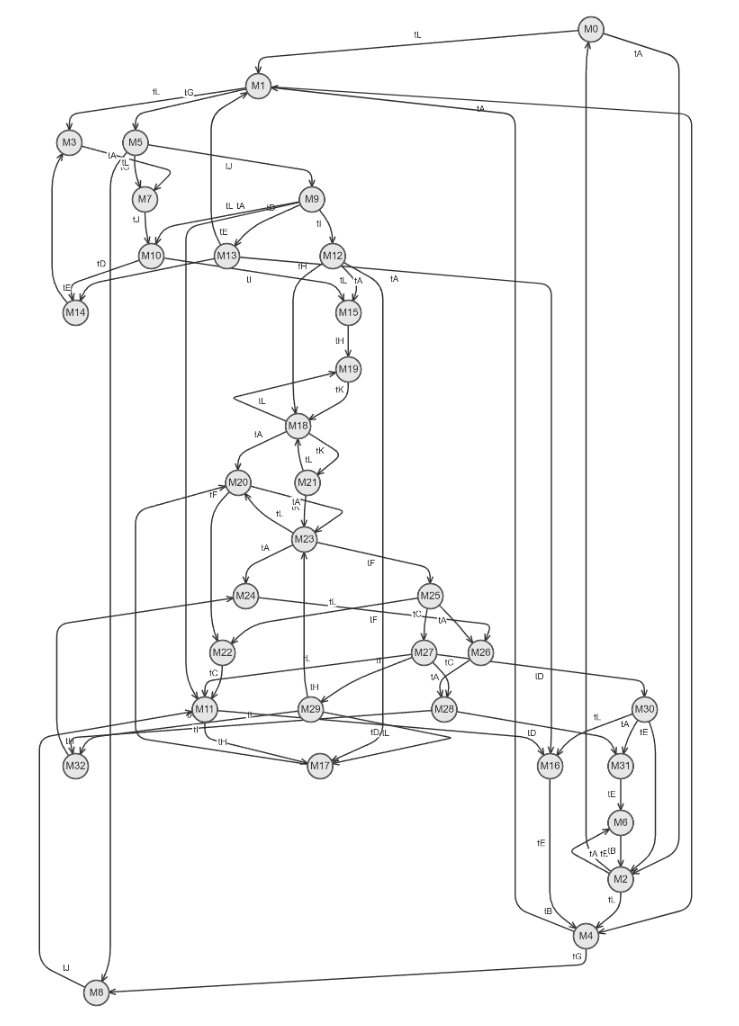
\includegraphics[width=0.8\textwidth]{assets/graphK2_auto}
    \caption{Graf dosažitelnosti pro k-omezenou síť s dvěma auty v křižovatce.}
    \label{fig:reachability_graph_k2}
\end{figure}

\begin{figure}[H]
    \centering
    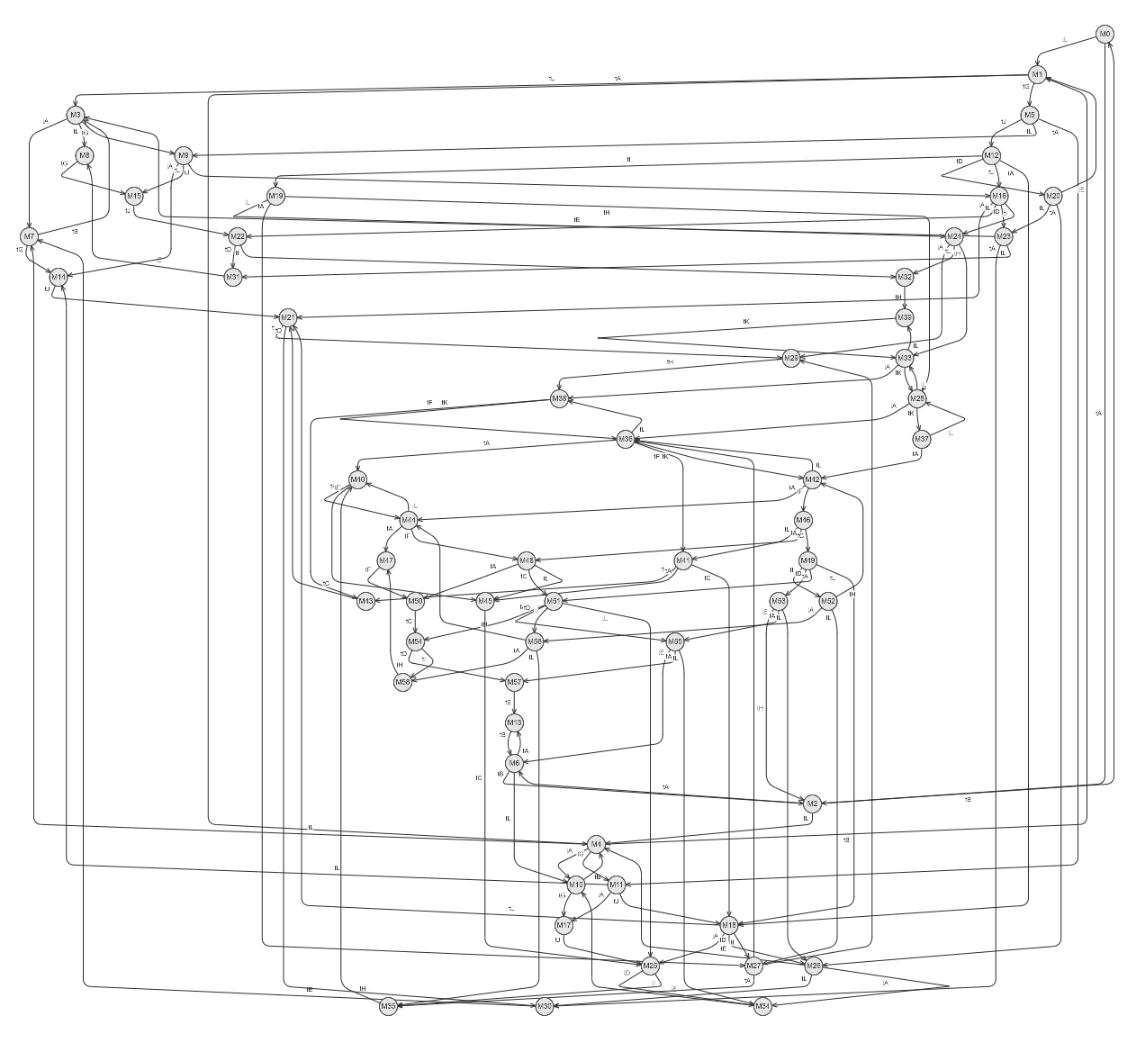
\includegraphics[width=1.0\textwidth]{assets/graphK3_auto}
    \caption{Graf dosažitelnosti pro k-omezenou síť s třemi auty v křižovatce.}
    \label{fig:reachability_graph_k3}
\end{figure}

\endinput

\newpage
\section*{Analýza sítě}
\label{sec:network_analyse}

V této sekci se budeme zabývat analýzou Petriho sítě, která reprezentuje chování semaforů na křižovatce.

\subsection*{P-Invarianty Petriho sítě}
\label{subsec:p_invariants}

\newcommand{\pI}  {0, 0, 0, 0, 0, 0, 1, 1, 0, 0, 1, 0, 0}
\newcommand{\pII} {0, 0, 1, 1, 0, 0, 0, 0, 0, 0, 0, 0, 1}
\newcommand{\pIII}{0, 1, 0, 0, 1, 0, 0, 0, 0, 0, 0, 0, 1}
\newcommand{\pIV} {0, 0, 0, 0, 0, 0, 1, 0, 1, 1, 0, 0, 0}
\newcommand{\pV}  {1, 0, 0, 0, 0, 1, 0, 0, 0, 0, 0, 1, 0}
\newcommand{\pAll}{1, 1, 1, 1, 1, 1, 2, 1, 1, 1, 1, 1, 2}

Pro tuto síť existuje celkem 5 p-invariantů vypsaných níže a výsledný p-invariant po sečtení všech hodnot je $Y_6$ = \orderArrayNumbered{\pAll}.\@
O všech p-invariantech můžeme říci, že jsou \textbf{minimální}, \textbf{netriviální} a \textbf{v kanonickém tvaru}.
A celkově tento systém p-invariantů je \textbf{úplný}.
Počáteční značení $M_0$ = (\orderArrayNumbered{\mO}).

\begin{table}[h!]
    \renewcommand{\arraystretch}{1.5}
    \resizebox{\textwidth}{!}{%
        \begin{tabular}{p{1cm} p{8cm} p{6cm}}%
            \ & \ul{Strukturální}                    & \ul{Systémové} \\
            \ & $Y_1^T$ - \orderArrayNumbered{\pI}   & $Y_1^T$ \cdot $M^0$ = 1 \\
            \ & $Y_2^T$ - \orderArrayNumbered{\pII}  & $Y_2^T$ \cdot $M^0$ = 1 \\
            \ & $Y_3^T$ - \orderArrayNumbered{\pIII} & $Y_3^T$ \cdot $M^0$ = 1 \\
            \ & $Y_4^T$ - \orderArrayNumbered{\pIV}  & $Y_4^T$ \cdot $M^0$ = 1 \\
            \ & $Y_5^T$ - \orderArrayNumbered{\pV}   & $Y_5^T$ \cdot $M^0$ = 3 \\
        \end{tabular}
    }
    \label{tab:p_invariants}
\end{table}
\vspace{-1em}

\subsection*{T-Invarianty Petriho sítě}
\label{subsec:t_invariants}

\newcommand{\tI}  {1, 1, 0, 0, 0, 0, 0, 0, 0, 0, 0, 0}
\newcommand{\tII} {0, 0, 0, 0, 0, 0, 0, 0, 0, 0, 1, 1}
\newcommand{\tIII}{0, 0, 1, 0, 0, 1, 0, 1, 1, 0, 0, 0}
\newcommand{\tIV} {0, 0, 0, 1, 1, 0, 1, 0, 0, 1, 0, 0}
\newcommand{\tAll}{1, 1, 1, 1, 1, 1, 1, 1, 1, 1, 1, 1}

Stejně tak zde nalezneme 4 t-invarianty, jejichž součet dává výsledný t-invariant \\$X_5$ = (\tAll).\@
Tyto invarianty jsou \textbf{minimální}, \textbf{netriviální} a \textbf{v kanonickém tvaru}.
Celkově tento systém t-invariantů je \textbf{úplný}.

\begin{table}[h!]
    \renewcommand{\arraystretch}{1.5}
    \resizebox{\textwidth}{!}{%
        \begin{tabular}{p{1cm} p{8cm} p{6cm}}%
            \ & \ul{Strukturální}   & \ul{Systémové} \\
            \ & $X_1^T$ = ({\tI})                                                    & $\sigma_1$ = $t_A$, $t_B$                \\[-5pt]
            \ & {\footnotesize pro $M^0$ = (3, 0, 1, 0, 0, 0, 0, 1, 0, 0, 1, 0, 1)}  &                                          \\[5pt]
            \ & $X_2^T$ = ({\tII})                                                  & $\sigma_1$ = $t_L$, $t_K$                \\[-5pt]
            \ & {\footnotesize pro $M^0$ = (3, 0, 0, 0, 1, 0, 1, 0, 1, 0, 0, 0, 0)}  &                                          \\[5pt]
            \ & $X_3^T$ = ({\tIII})                                                   & $\sigma_1$ = $t_F$, $t_C$, $t_I$, $t_H$  \\[-5pt]
            \ & {\footnotesize pro $M^0$ = (3, 0, 0, 0, 1, 0, 1, 0, 1, 0, 0, 0, 0)}  &                                          \\[5pt]
            \ & $X_4^T$ = ({\tIV})                                                   & $\sigma_1$ = $t_G$, $t_J$, $t_D$, $t_E$  \\[-5pt]
            \ & {\footnotesize pro $M^0$ = (3, 0, 1, 0, 0, 0, 0, 1, 0, 0, 1, 0, 1)}  &                                          \\
        \end{tabular}
    }
    \label{tab:t_invariants}
\end{table}
\vspace{-1em}

\newpage
\subsection*{Vlastnosti PN systému}
\label{subsec:pn_properties}

Za pomocí P a T invariantů můžeme o síti říci tyto vlastnosti:

\begin{itemize}
    \item Síť je \textbf{konzervativní}, protože existuje p-invariant pokrývající všechny stavy. \\ $Y_6$ = \orderArrayNumbered{\pAll}
    \item Síť je \textbf{\ut{striktně} repetiční} protože existuje t-invariant pokrývající všechny přechody. \\ $X_5$ = (\tAll)
    \item Síť je \textbf{k-omezená} pro k = 3, kde k je maximální počet aut pohybující se v křižovatce.
    \item {
        Síť je \textbf{bezpečná} pouze pro vnitřní komponentu systému křižovatky.
        Celý systém je \textbf{bezpečný} v momentě, kdy je síť omezena pro maximálně 1 auto.
    }
    \item Síť je \textbf{živá}, vzhledem k vytvořenému grafu dosažitelnosti pro výchozí značení.
    \item Síť je \textbf{reverzibilní}, protože dle grafu dosažitelnosti neexistuje stav, ze kterého by se nedalo dostat zpět do výchozího značení.
\end{itemize}

\endinput

\section*{Závěr}
\label{sec:summary}

Vytvořená Petriho síť přesně modeluje chování semaforů na křižovatce, čímž poskytuje robustní základ pro analýzu a návrh systémů řízení dopravního toku.
Simulace ověřily, že model zajišťuje bezpečné a spolehlivé střídání světelných signálů v obou směrech provozu.

Navržený model je připraven k dalšímu rozvoji, například k začlenění adaptivního řízení na základě aktuálního dopravního zatížení nebo integraci přechodů pro chodce.
Během analýzy bylo zjištěno, že při zvýšení maximálního počtu vozidel na křižovatce dochází k expanzivnímu růstu grafu dosažitelnosti (viz \tabref{tab:reachability_count}), což však nemá negativní dopad na funkčnost nebo vlastnosti samotné sítě.

\endinput

\end{document}